% D.39 直线 y = -3/4 x + 3，A 在 x 轴(4,0)，B 在 y 轴(0,3)；P 在 AB 上，过 P 作 x 轴垂线 PQ；矩形 OQPM
\documentclass[tikz,border=4pt]{standalone}
\usepackage{ctex}
\usepackage{amsmath}
\usetikzlibrary{calc}
\begin{document}
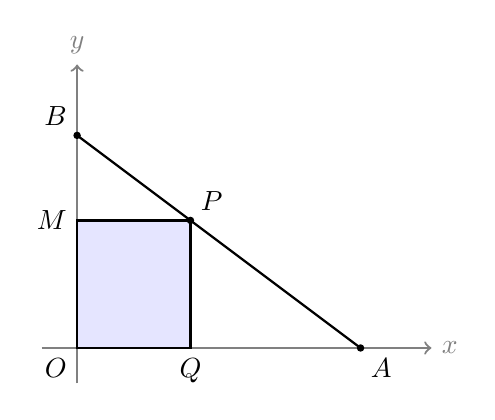
\begin{tikzpicture}[scale=0.9, thick]
  \draw[gray, ->] (-0.5, 0) -- (5, 0) node[right] {$x$};
  \draw[gray, ->] (0, -0.5) -- (0, 4) node[above] {$y$};
  \coordinate (A) at (4, 0);
  \coordinate (B) at (0, 3);
  \draw (A) -- (B);
  \coordinate (Q) at (1.6, 0);
  \coordinate (P) at (1.6, 1.8);
  \coordinate (M) at (0, 1.8);

  \fill[blue!10] (0,0) -- (Q) -- (P) -- (M) -- cycle;
  \draw (0,0) -- (Q) -- (P) -- (M) -- cycle;

  \fill (A) circle (1.5pt); \node[below right] at (A) {$A$};
  \fill (B) circle (1.5pt); \node[above left]  at (B) {$B$};
  \fill (P) circle (1.5pt); \node[above right] at (P) {$P$};
  \node[below] at (Q) {$Q$};
  \node[left]  at (M) {$M$};
  \node[below left] at (0,0) {$O$};
\end{tikzpicture}
\end{document}
